\section{Phase 1: Discover}

During the discovery phase, the team organized its structure, established roles for management, conducted research and developed initial proposals for the module.

\subsection{Team Organization}

Our team is composed of five students:
\begin{itemize}
    \item \textbf{Ermelinda Giulivo}
    \item \textbf{Rafael Monllor Ballesteros}
    \item \textbf{Daniel Mauricio Ruiz Suarez}
    \item \textbf{Jurij Diego Scandola}
    \item \textbf{Abdul Moiz}
\end{itemize}

The team leader and \textbf{Backbone member} is Jurij Diego Scandola.

Our responsibilities and roles are:
\begin{itemize}
    \item \textbf{Rapporteur}: Rafael Monllor Ballesteros
    \item \textbf{Schedule manager}: Jurij Diego Scandola
    \item \textbf{Art director}: Daniel Mauricio Ruiz Suarez
    \item \textbf{Tech manager}: Ermelinda Giulivo
    \item \textbf{Designer}: Abdul Moiz
\end{itemize}

\subsection{Project Management}

Our team plans to solve the tasks according to the following GANTT:

\begin{figure}[H]
    \centering
    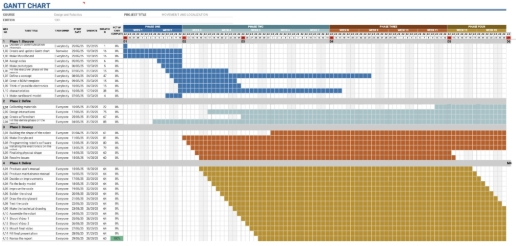
\includegraphics[width=\linewidth]{../ReportMovementModule/images/Aspose.Words.728084da-df58-4b9d-a372-f65cffbdb23d.001.jpeg}
    \caption{Project GANTT Chart}
\end{figure}

\subsection{Research}

The research phase is a critical foundation for the development of the movement and localization module of the indoor robot. At this stage, the primary objective is to explore and analyse existing technologies, methodologies and systems that enable precise navigation and positioning within indoor environments. Unlike outdoor settings, indoor environments present unique challenges such as signal attenuation, dynamic obstacles and limited access to GPS, making robust and reliable localization and movement a complex task.
